\section{Method}
\label{sec:3_method}
\subsection{Data Acquisition}
The pipelines for our data acquisition are illustrated in \autoref{fig:data_acq}. We start with the transfer records webpages on \href{www.transfermarkt.co.uk}{Transfermarkt}, collecting 500 records for each year from 2005 to 2023. Using the Rcrawler package to loop through URLs across years and pages, we extract the main pages of all players associated with these records. From the player pages, Rcrawler is then used to fetch the URLs of rumor pages, which contain all relevant rumor posts about the player. By identifying the corresponding nodes with Selector Gadget and using the rvest package, we scrape the rumor source, the posting date, and the user-summarized content of each rumor. For ground truth data, we dynamically request the player's transfer records page to obtain JSON-formatted transfer histories. Using the jsonlite package, we convert this data into a data frame for further alignment and analysis.
\begin{figure}[ht]
    \centering
    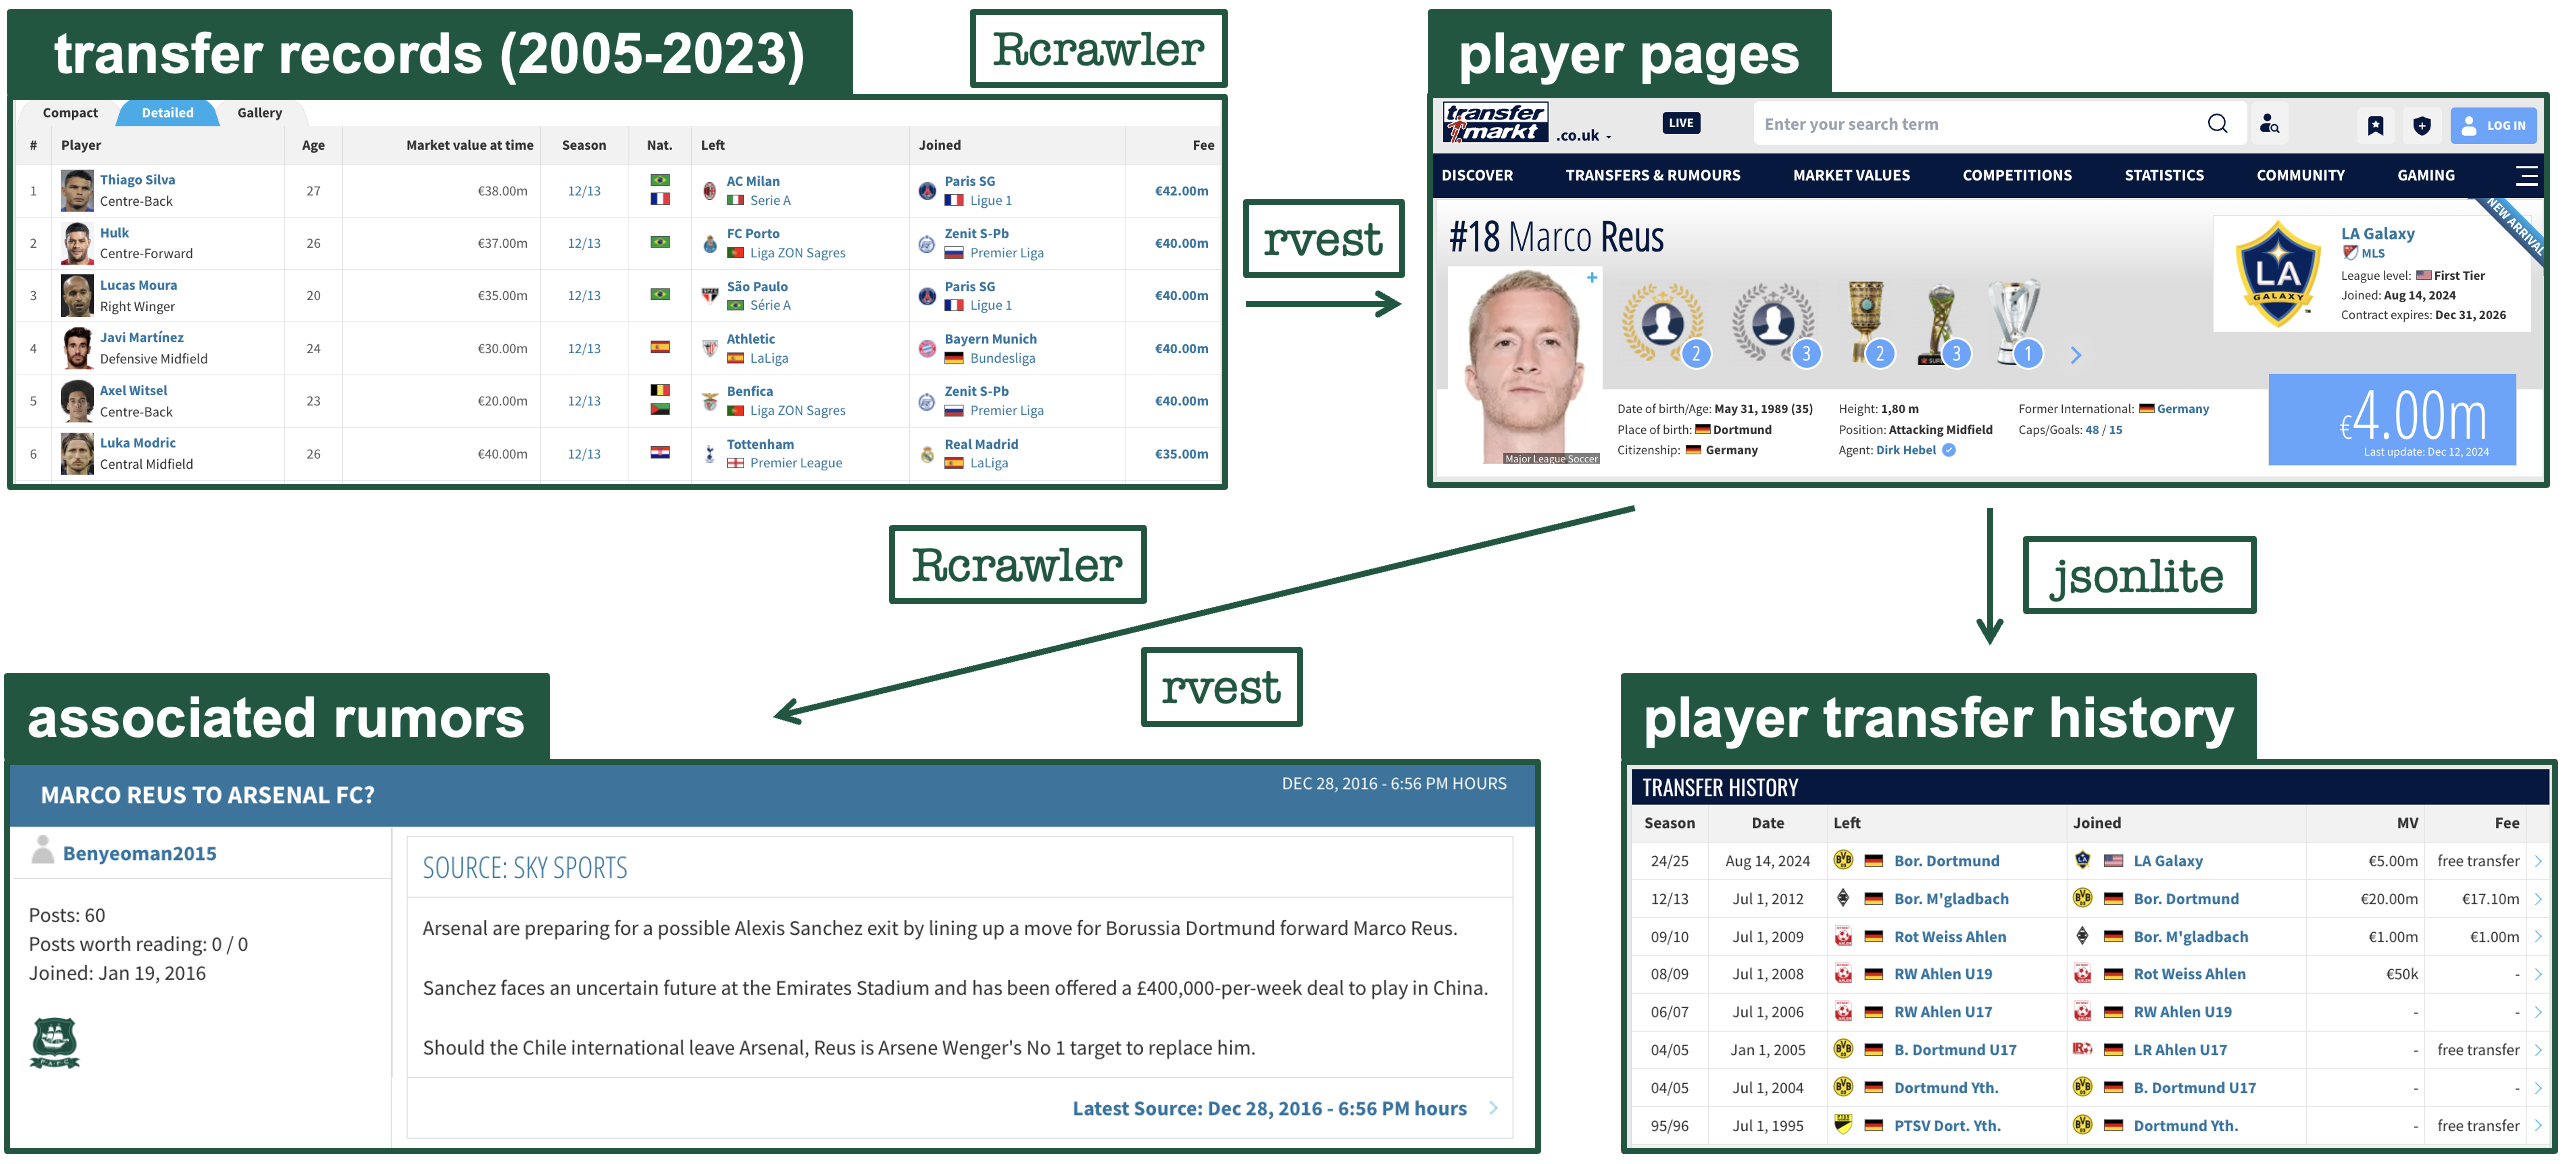
\includegraphics[width=.8\textwidth]{figs/data_acq.png}
    \caption{
        Pipelines for Data Acquisition
    }\label{fig:data_acq}
\end{figure}

\subsection{Text Processing}
To evaluate the confidence expressed in rumor posts about potential transfers, we aimed to create a quantified metric (\autoref{fig:text_proc}). Initially, we used the \texttt{get\_sentiment()} function from the Syuzhet package in R, a dictionary-based method that detects words with specific attitudes and assigns a positivity score, which is then summed for the entire paragraph. However, this method is unable to accurately assess the confidence regarding a specific player's transfer to a particular club and is overly influenced by irrelevant or redundant parts of the posts. To address these limitations, we integrated the ChatGPT 3.5 turbo API. By structuring the post content into a designed prompt, we utilized the language model to generate a graded numerical evaluation of confidence and return in JSON format.
\begin{figure}[ht]
    \centering
    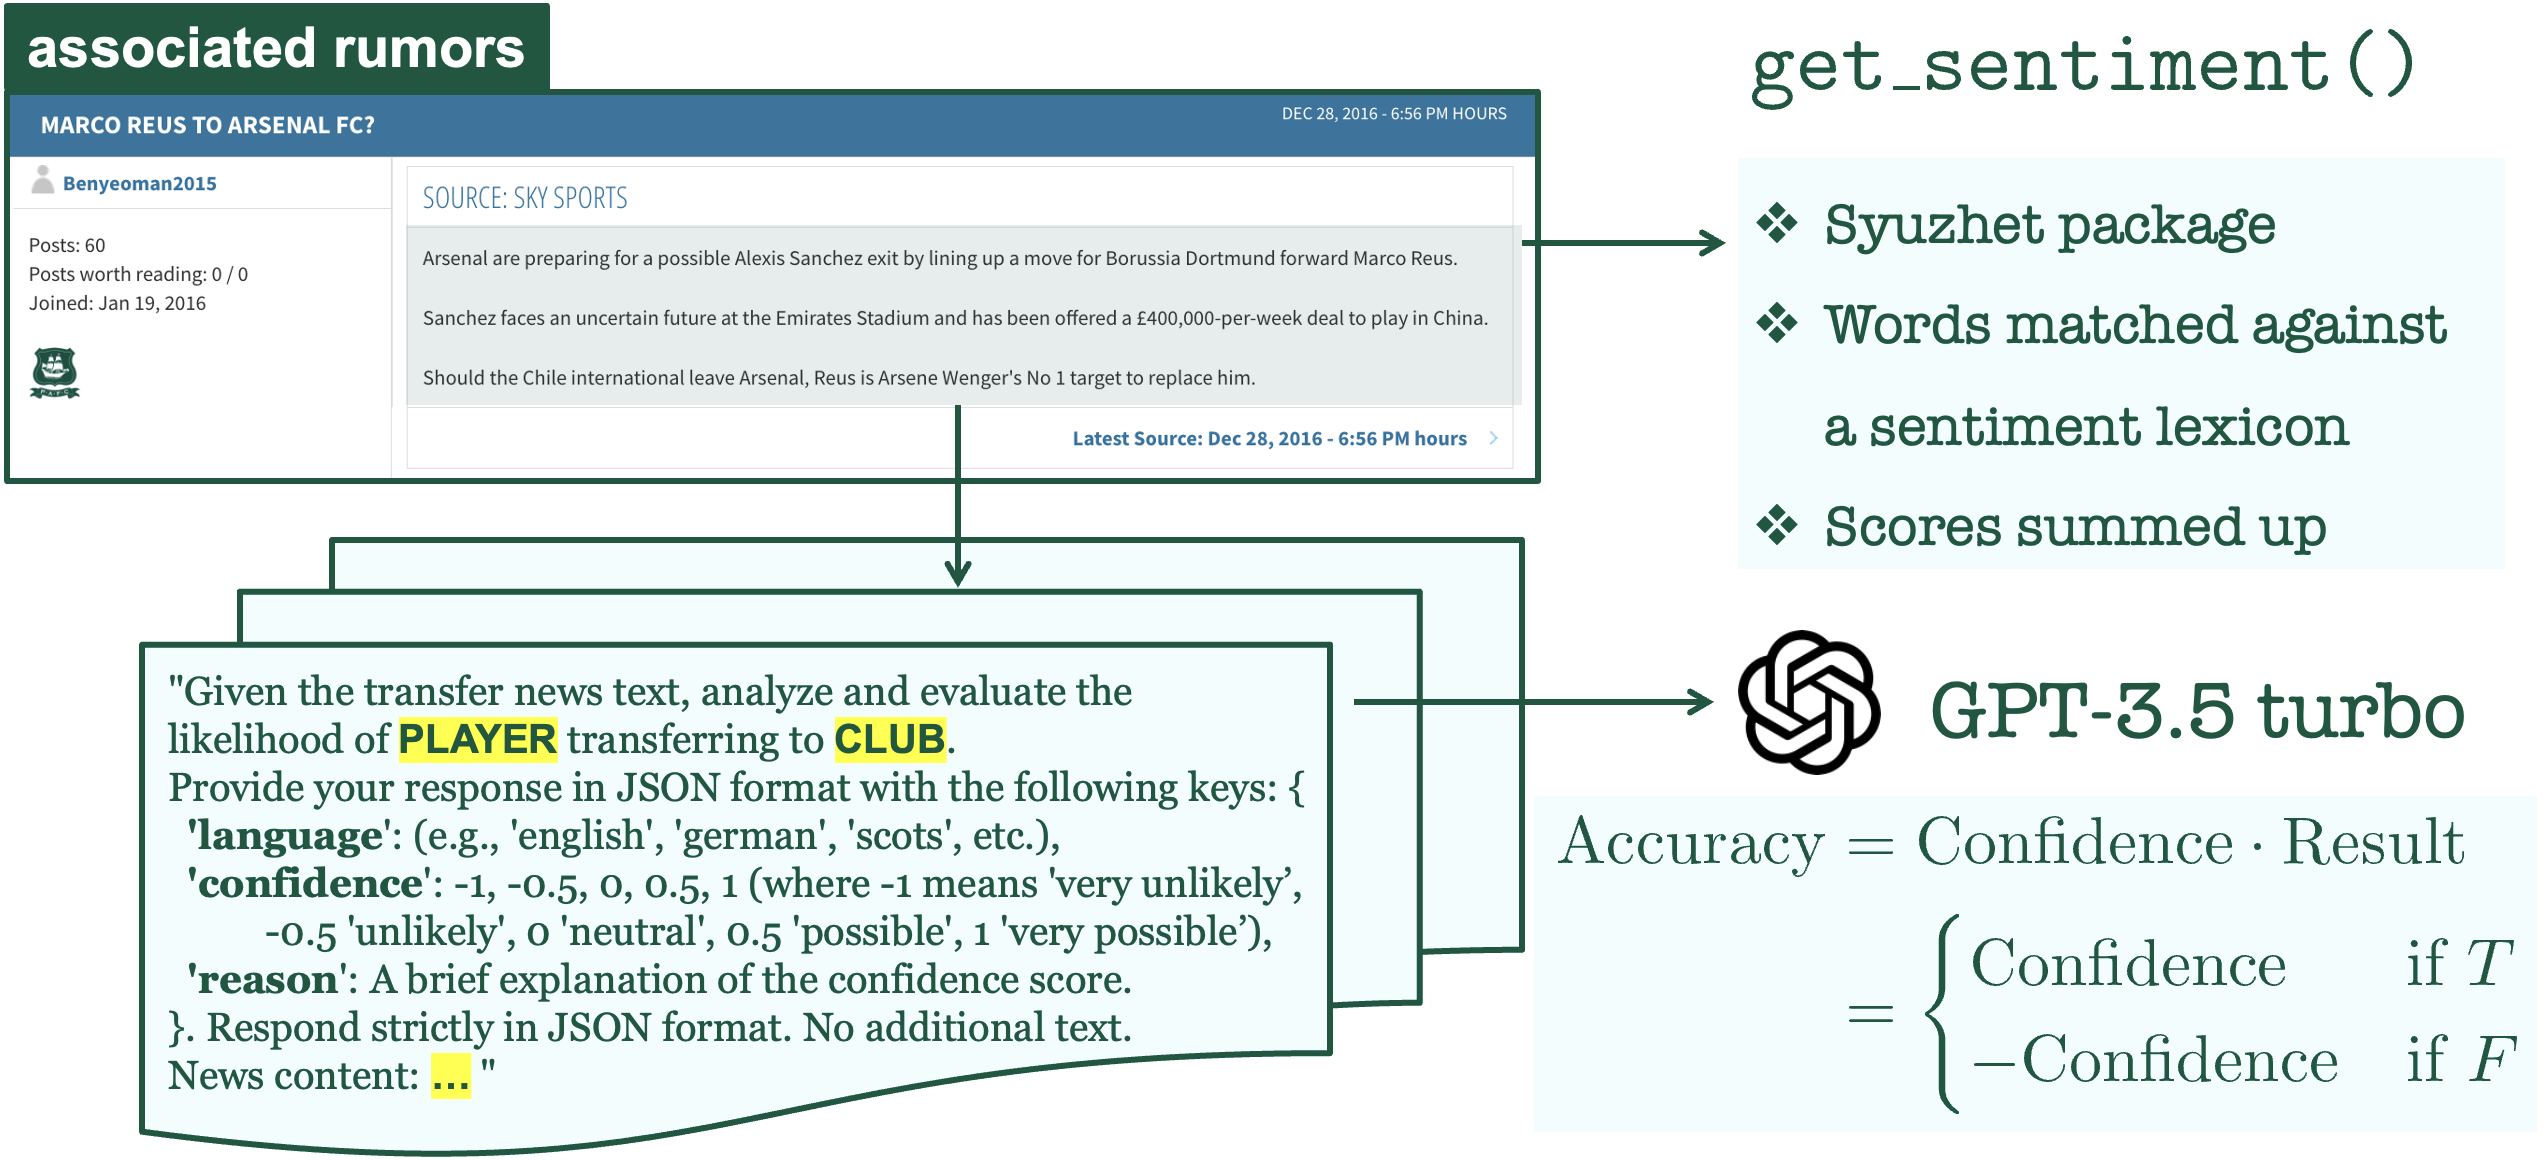
\includegraphics[width=.8\textwidth]{figs/text_proc.png}
    \caption{
        Framework for Analyzing Confidence in Transfer Rumor Contents
    }\label{fig:text_proc}
\end{figure}

\subsection{Data Alignment}


\subsubsection{Source Name Alignment}
 % URL 不统一,有些是网址(格式不一,如 https://www.theguardian.com, www1.bbc.com),有些是 source 名称而非具体网址(如 Source: Guardian, Source: L´Equipe),如\autoref{fig:align_metd}
 % 对于非具体网址的,通过 谷歌搜索引擎搜索关键词,将 First Organic Search Result 的结果作为网址(人工验证,这种方法很可靠)
 % 对于具体网址但格式不同的,通过正则匹配等方式格式化
The source names we get from rvest are not standardized and mainly consists of two types: URLs (e.g. \url{www.theguardian.com}, \url{www1.bbc.com}) and specific names (e.g. Guardian, L´Equipe). 

For specific names, we used Google to search for keywords that showed up in the names. By using the First Organic Search Result as our target answer, we are able to get reliable and consistent standardized URL results that had undergone manual double-check.

For URLs, the main problem is that the same rumor source can have different URLs and domain names (e.g. m.bbc.com, www.bbc.co.uk). Our first step is to match the URL start (https://) and delete subdomain name (e.g. www./en./m.) that appear before the actual information. Then we match and delete top domain name that appear at the end of the URL. All URLs are processed using regex expressions in R.

% 最终统一格式为 https://xxx
The final result we get for rumor source are formatted as https://xxx and is easy for further data processing.

\subsubsection{Rumor-Fact Alignment}

% 如\autoref{fig:align_metd},谣言和事实匹配,当且仅当球员的名字相同,且时间上落入给定的区间(rumor发布之后的XXX月内)。若谣言匹配上某个事实,但目标 club 不同,则说明谣言有误;若未匹配,同样说明谣言有误(球员实际未转会)

% 首先,球员的名字是唯一的,谣言和事实对于这个词条是一致的,直接通过小写化、去除特殊字符(短横线等),如果名字相同,则名字匹配上。

% 俱乐部的名字较为多样,不规范,需要经过较为复杂的 rectify(如去除尾部的表示俱乐部、协会等常用词及其缩写、去除部分表示地域的缩写、恢复拉丁转写等)。经过复杂的 rectify,如果对得上,则说明俱乐部对得上。

% 时间上,两条相互匹配的事实和谣言,事实必须是在谣言之后发生的。同时,如果一个谣言匹配上了多条事实,可能是因为该球员发生了不止一次转会,因此取最近的一条事实记录作为谣言对应的事实。

The alignment of rumors and facts is determined based on two main criteria: the player's name and the timing of the event, as illustrated in \autoref{fig:align_metd}. A rumor and fact are considered aligned if and only if the player's name matches and the event occurs within a specified time frame (e.g., within a few months following the publication of the rumor). If the player's name matches but the target club differs, the rumor is deemed incorrect. Similarly, if no match is found between the rumor and the fact, the rumor is also classified as incorrect, indicating that the player did not actually transfer.

First, the player’s name serves as a unique identifier, ensuring consistency between the rumor and the corresponding fact for that entry. A direct match is obtained by standardizing the name, which involves converting it to lowercase and removing special characters (such as hyphens). If the resulting names are identical, they are considered to match.

In contrast, club names exhibit greater variability and inconsistency, necessitating a more intricate rectification process. This process includes removing common suffixes that denote clubs or associations, addressing regional name abbreviations, and restoring Latin transliterations. After applying this rectification, a match between clubs indicates that the club associated with the rumor is accurate.

Regarding timing, the rumor and corresponding fact must satisfy the condition that the fact occurs after the rumor. Furthermore, if a rumor is associated with multiple facts, it may suggest that the player underwent multiple transfers. In such cases, the most recent fact, in terms of its proximity to the rumor, is selected as the corresponding fact.


\begin{figure}[ht]
    \centering
    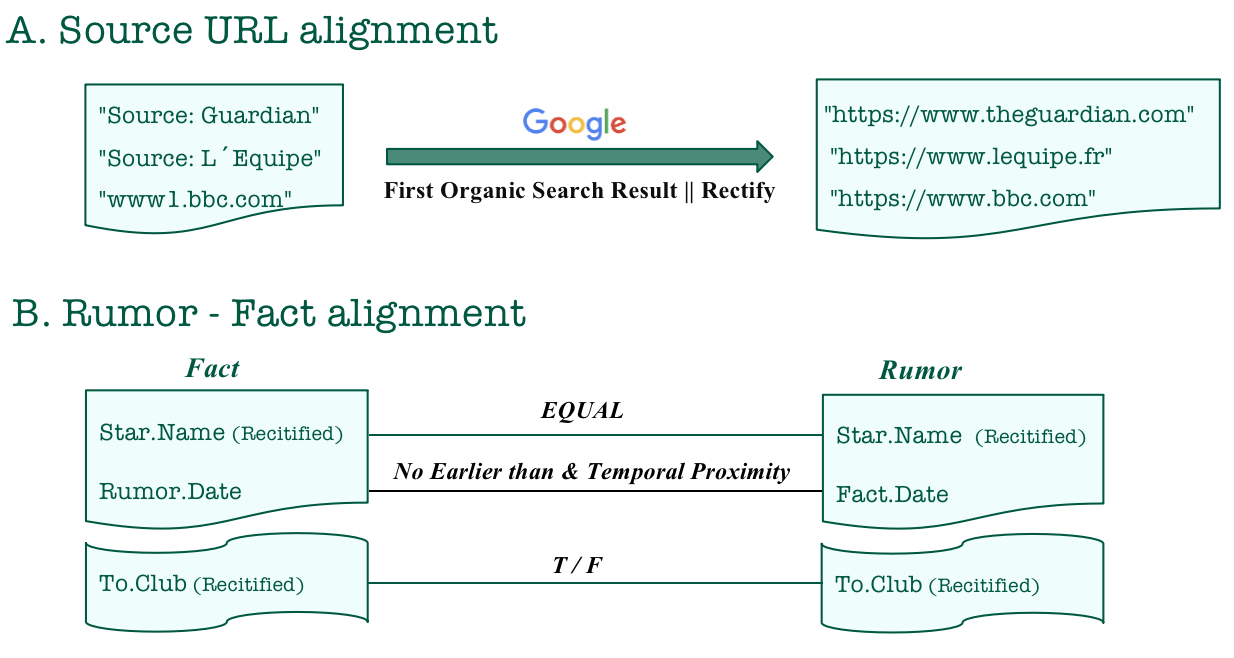
\includegraphics[width=.6\textwidth]{figs/align_metd.png}
    \caption{
        Methods for alignment
    }\label{fig:align_metd}
\end{figure}

\subsection{Feature Engineering}

% 这部分我们将分析时间、可靠性指标、content and source,等数据特征,筛选出对预测更有用、且更具可解释性的特征

In this section, we will analyze data features such as time, reliability indicators, content, and source, and select those that are more useful for prediction and offer greater interpretability.

\subsubsection{Time}

% 时间包括月份、星期、小时、分钟。做出箱线图,如 \autoref{fig:time_boxplot},我们发现有且仅有月份与准确度存在明显的非线性关系。

% 进一步构建随机森林模型,计算 increased accuracy(每个特征对 accuracy 的共享),如\autoref{fig:time_acc},可见月份对模型预测的共享确实显著强于其它的,进一步验证了猜想。

% 可能是因为赛季转会存在周期,距离实际转会时间越远的谣言越不容易对。
% % 与可视化结果对应

Time encompasses various units, including month, week, hour, and minute. As illustrated in \autoref{fig:time_boxplot}, a significant nonlinear relationship between the month and accuracy was observed.

Additionally, by constructing a random forest model to evaluate the contribution of each feature to the accuracy (i.e., the share of each feature in the model's predictive power), as shown in \autoref{fig:time_acc}, it is evident that the month significantly outperforms other features in terms of its impact on prediction accuracy. This further supports the hypothesis that the month is a key factor in determining the accuracy of transfer rumors.

This is likely due to the cyclical nature of transfer seasons, wherein rumors occurring farther from the actual transfer period tend to be less accurate.


\begin{figure}[ht]
    \centering
    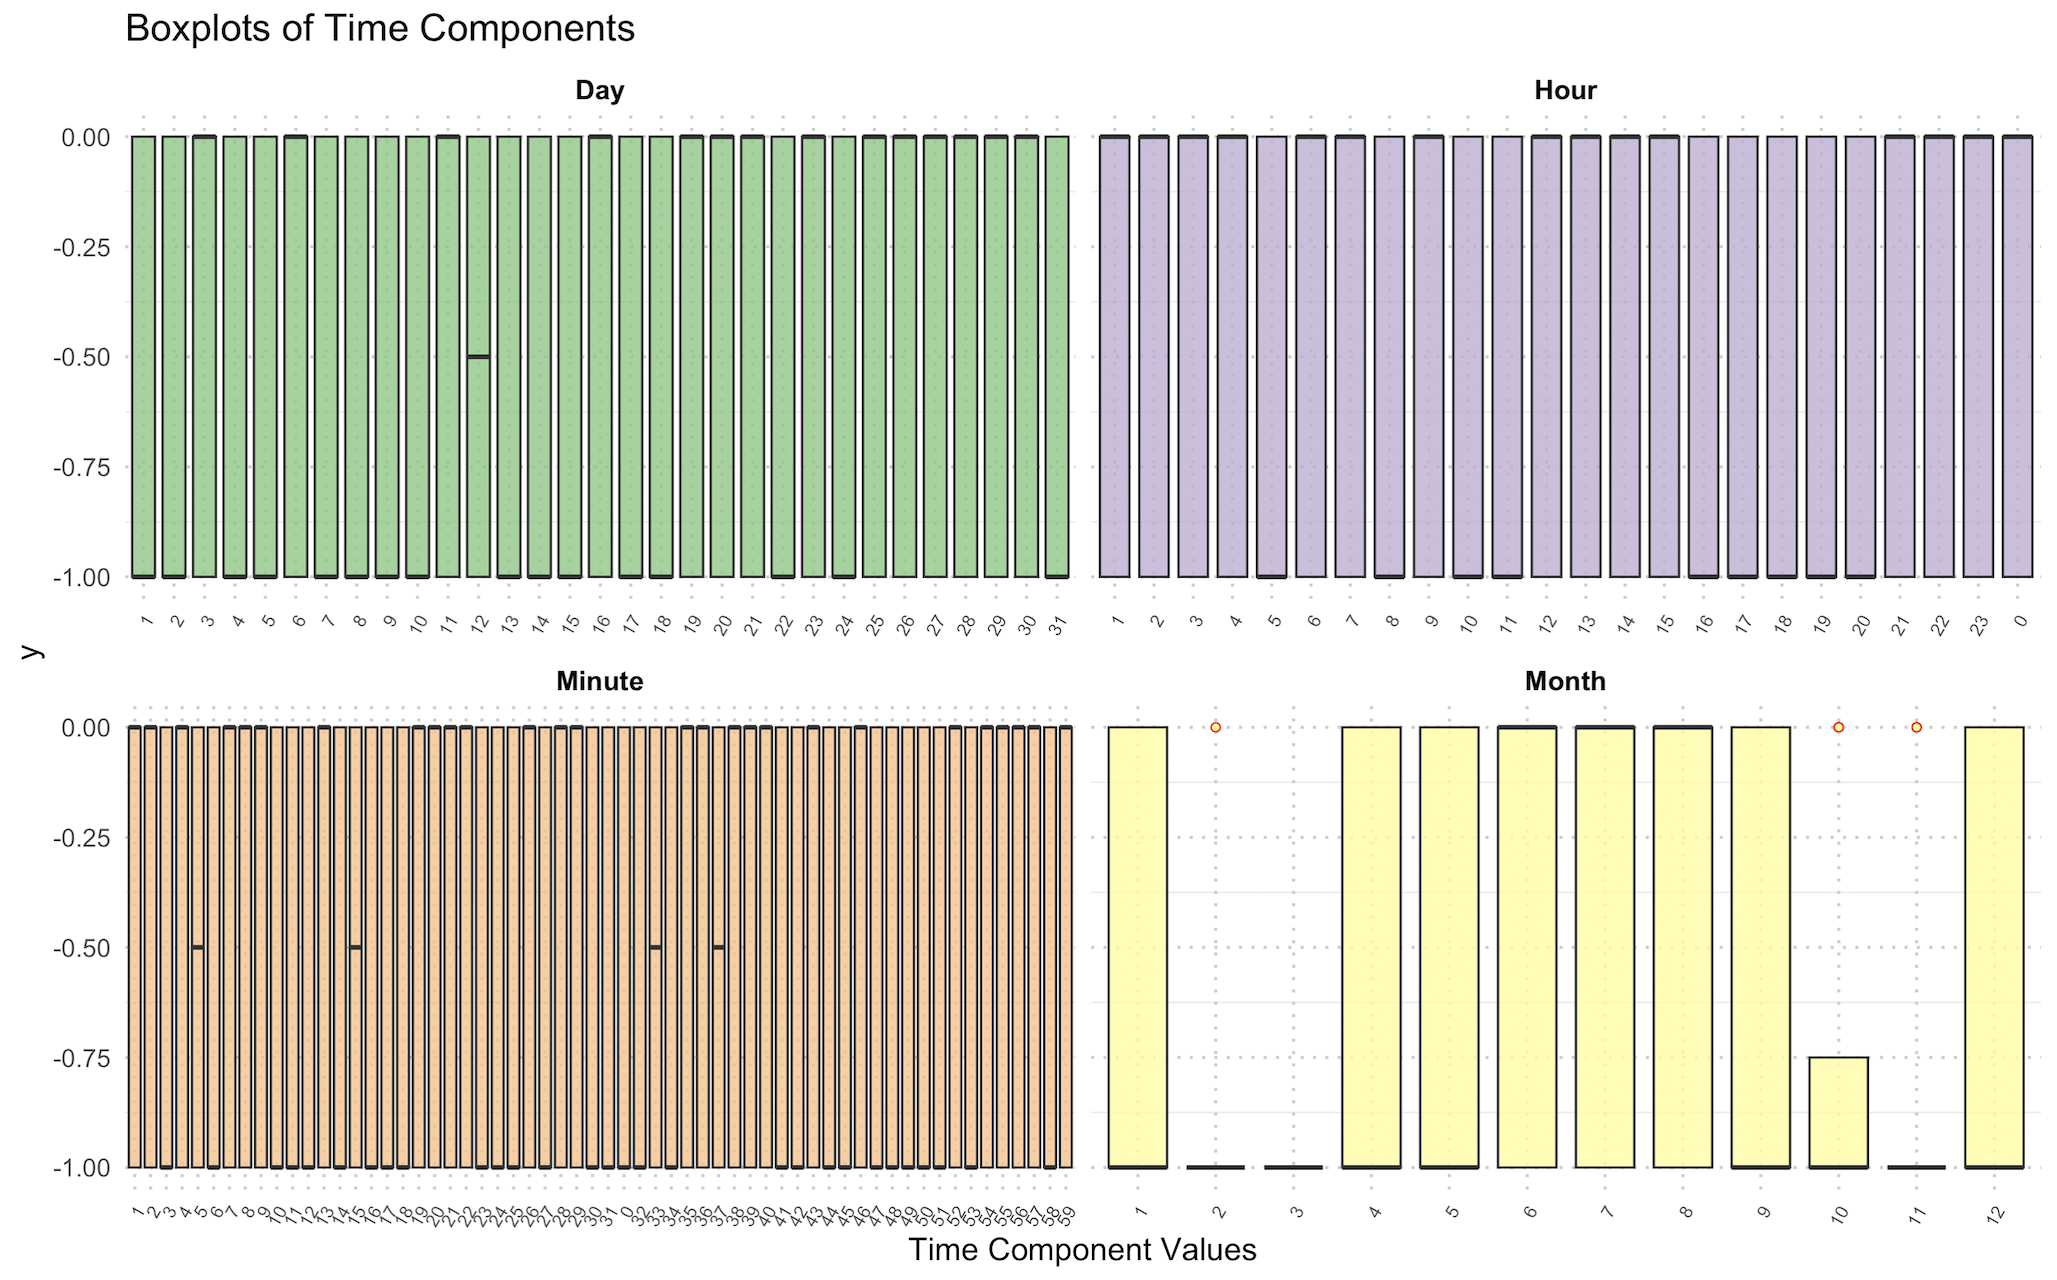
\includegraphics[width=.8\textwidth]{figs/time_boxplot.png}
    \caption{
       Time Boxplot
    }\label{fig:time_boxplot}
\end{figure}

\begin{figure}[ht]
    \centering
    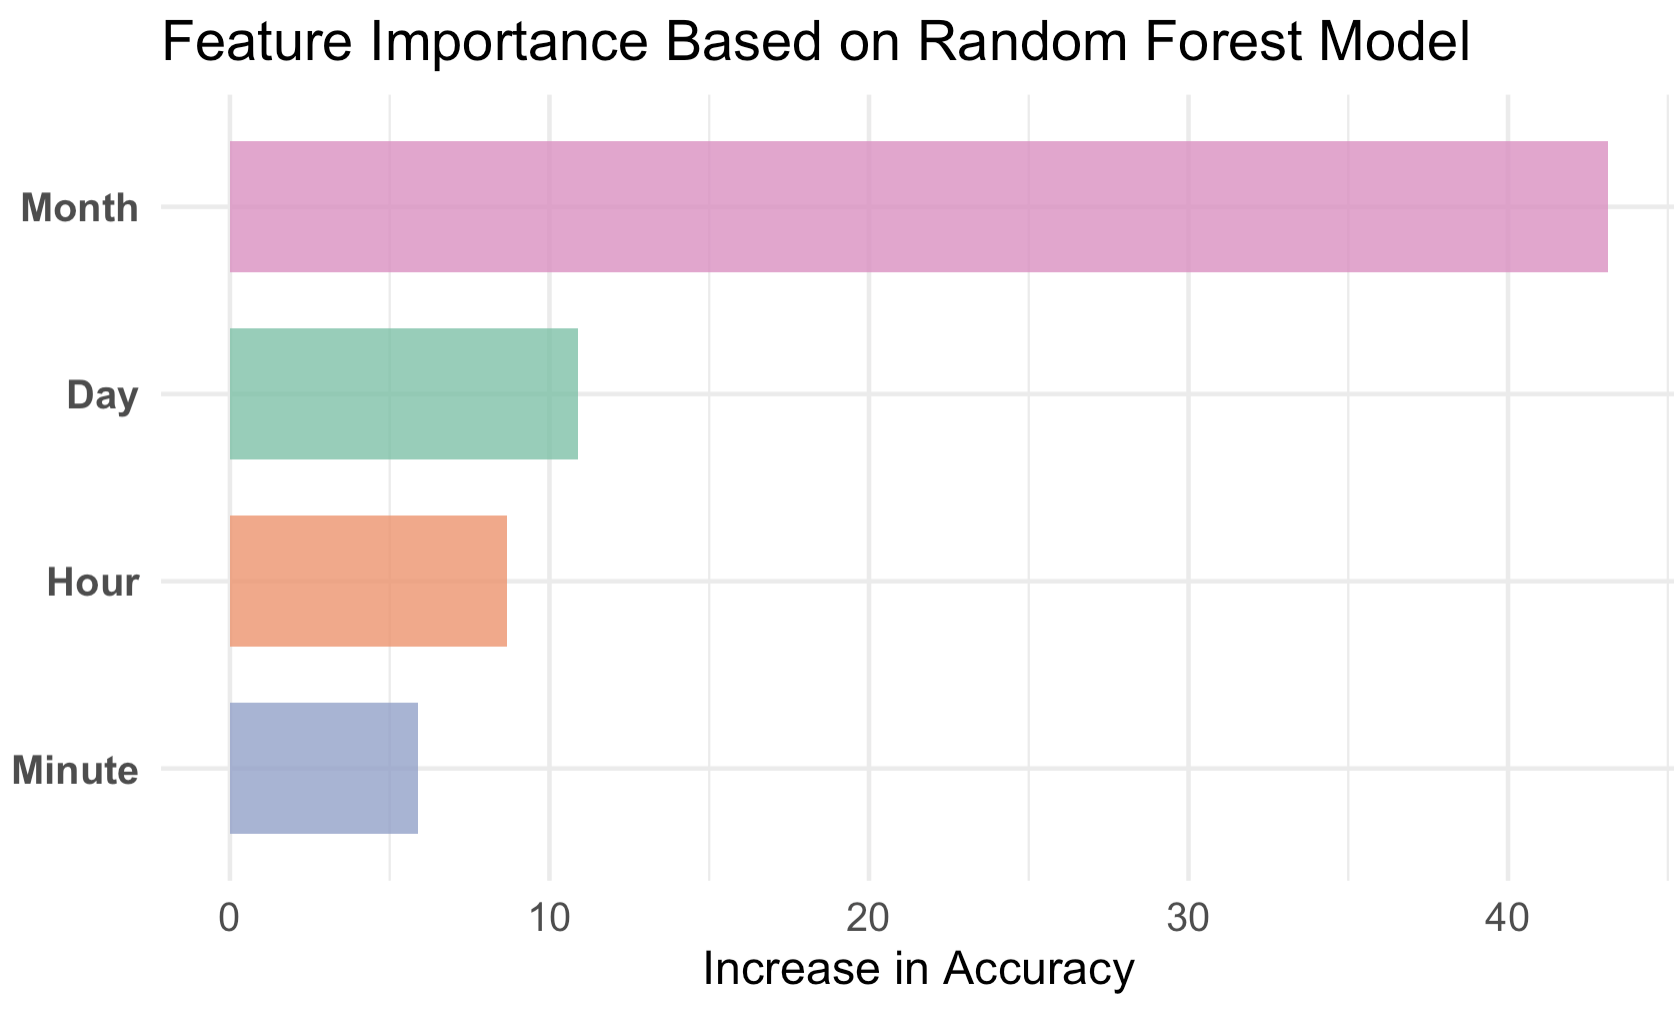
\includegraphics[width=.5\textwidth]{figs/time_acc.png}
    \caption{
       Increased accuracy for Time
    }\label{fig:time_acc}
\end{figure}

\subsubsection{Reliability}

Variable Correlation:

\begin{itemize}
    \item \textbf{GPT.confidence}: 0.24611174
    \item \textbf{Rumor.Sentiment}: -0.03115098
\end{itemize}



% GPT.confidence相比于Rumor.Sentiment,与谣言真实性的相关程度明显很多。

% 进一步可视化,如\autoref{fig:senti_cor},发现Rumor.Sentiment确实与谣言真实性没有明显线性或非线性关系,而GPT.confidence则明显正相关

% 可能是因为Rumor.Sentiment的生成方式只考虑了局部的语义,而GPT.confidence则能捕捉到全局语义。或者,GPT 通过预训练掌握了更多的先验知识。

GPT.confidence exhibits a significantly stronger correlation with the truthfulness of rumors compared to Rumor.Sentiment.

Further analysis, as depicted in \autoref{fig:senti_acc}, shows that Rumor.Sentiment lacks any discernible linear or nonlinear relationship with the truthfulness of the rumor. In contrast, GPT.confidence displays a clear positive correlation.

This disparity may arise because Rumor.Sentiment primarily reflects local semantics, focusing on the sentiment within the immediate context of the rumor. On the other hand, GPT.confidence incorporates global semantics, capturing broader contextual information. Additionally, GPT's pre-training likely provides it with a richer base of prior knowledge, which could enhance its ability to assess the truthfulness of rumors.

\begin{figure}[ht]
    \centering
    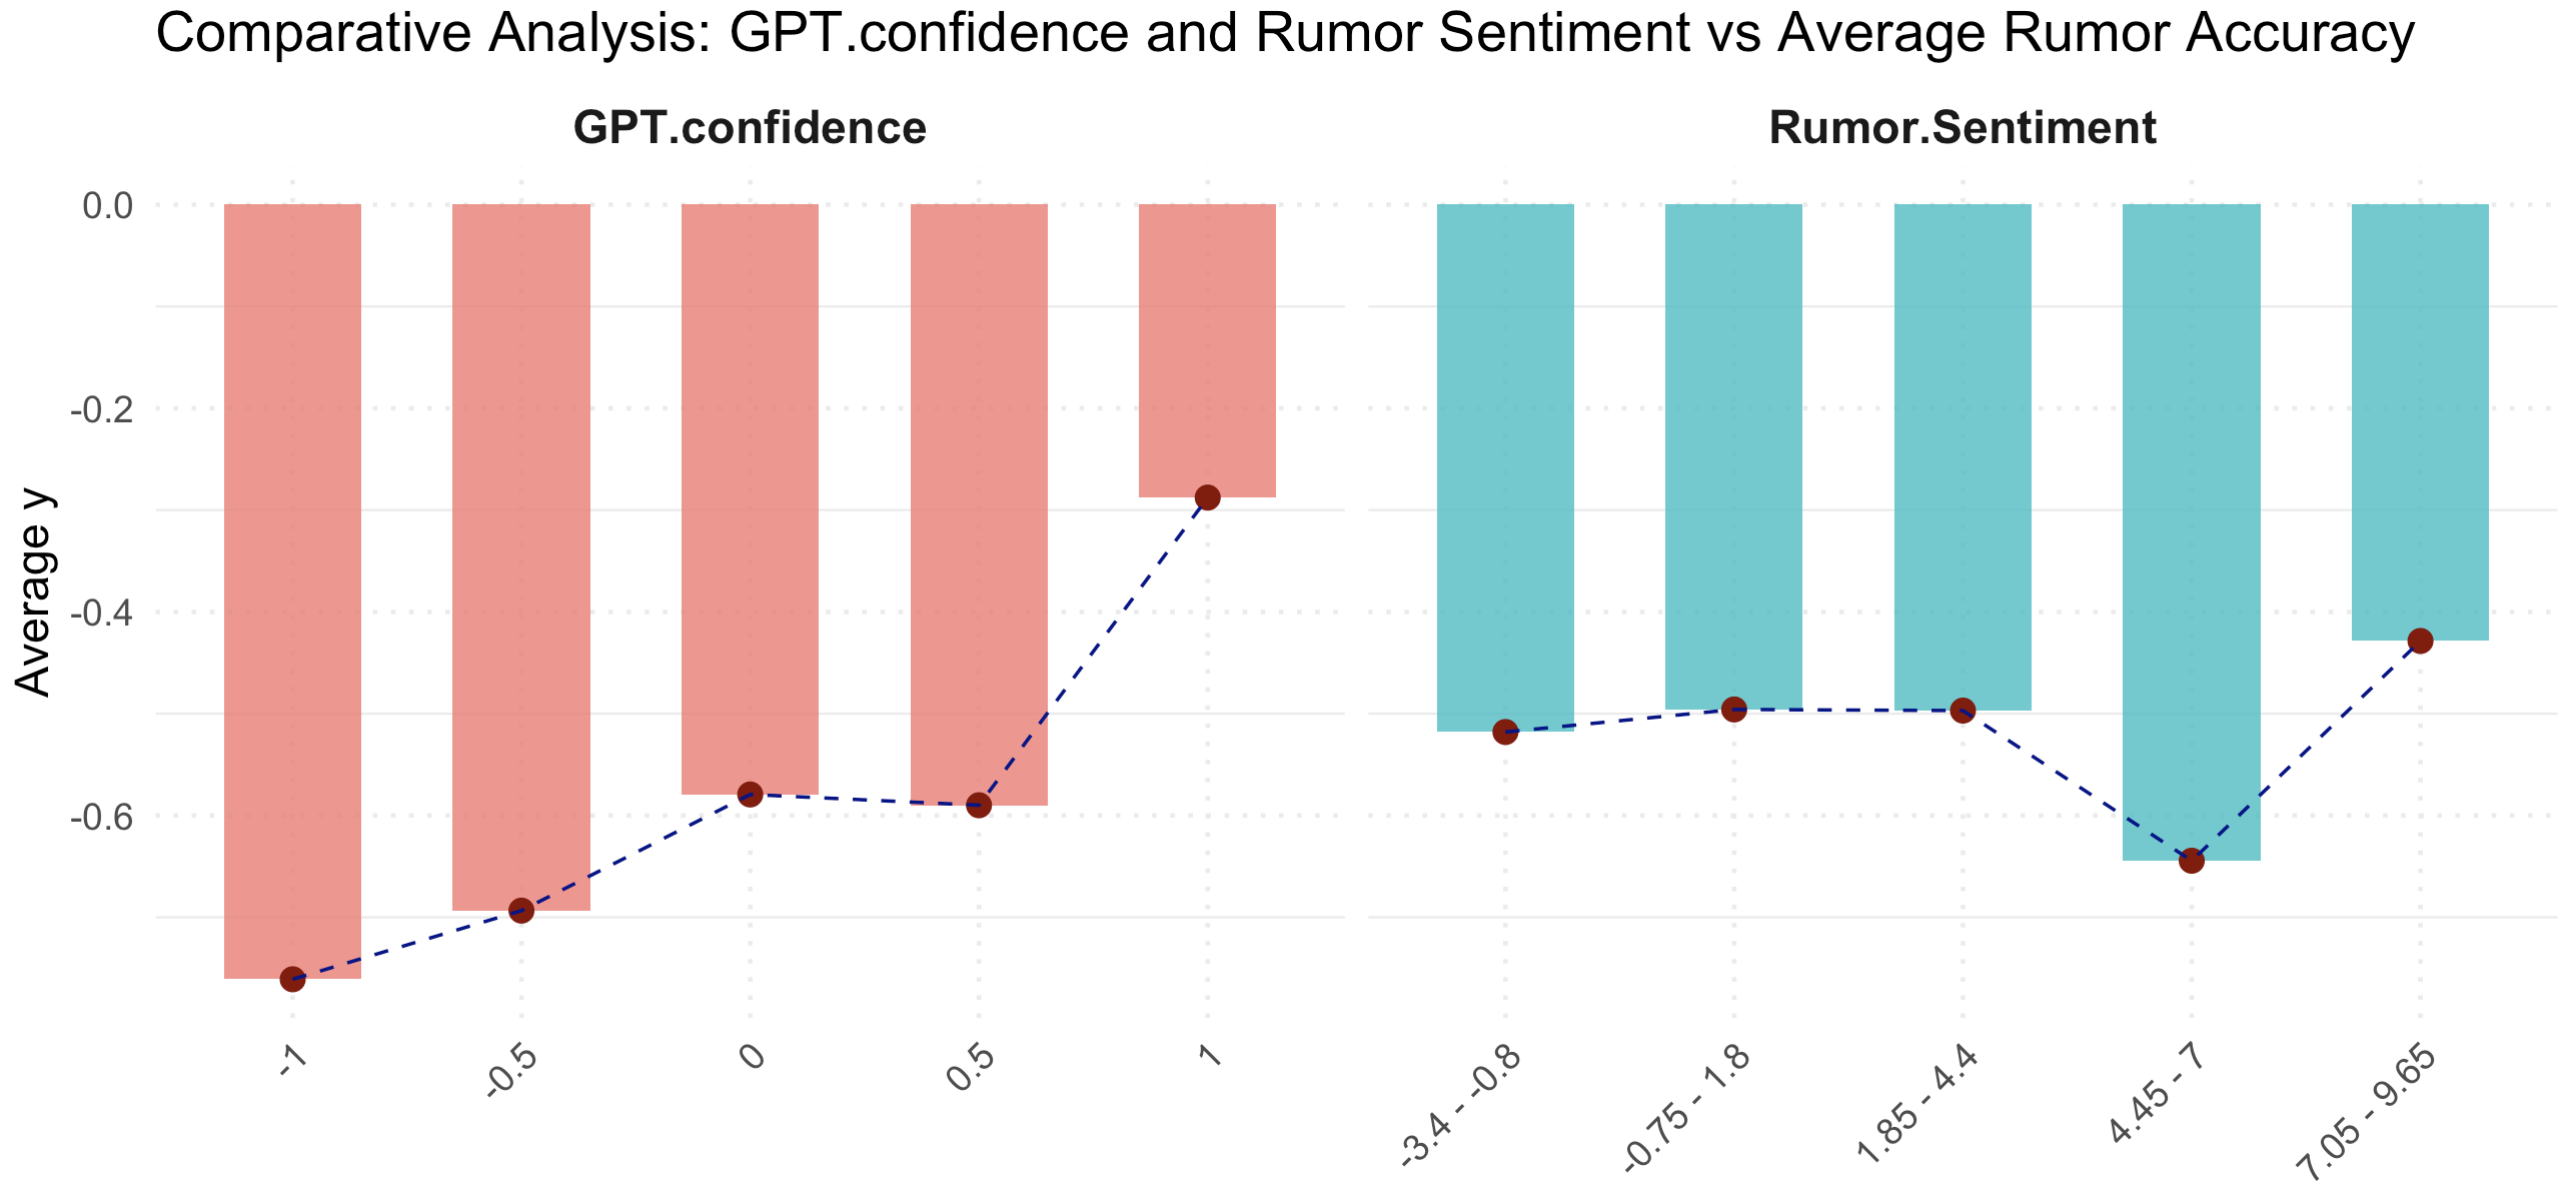
\includegraphics[width=.8\textwidth]{figs/senti_acc.png}
    \caption{
       Correlation between reliability and truthfulness % The left part of the figure needs to be redrawn
    }\label{fig:senti_acc}
\end{figure}

\subsubsection{Rumor Content and Source}

When using only the rumor content as a feature, we construct a random forest model to evaluate its contribution to increased accuracy (i.e., the proportion of each feature's influence on model accuracy), as shown in \autoref{fig:cont_acc}.

Interpretative analysis:

\begin{itemize}
    \item \textbf{united / manchester / chelsea / arsenal / liverpool / city:} These terms refer to well-known football clubs (e.g., Manchester United, Manchester City, Chelsea, Arsenal, etc.). The frequency of their occurrence in transfer rumors may be correlated with the prominence of these teams. Rumors involving popular clubs often attract more attention, leading to higher likelihoods of verification and appearing in more credible news sources. 
    \item \textbf{deal / transfer / loan / fee:} These words describe essential aspects of transfer transactions (such as deal, transfer, loan, transfer fee). Rumors that include specific details about transfers tend to be perceived as more credible, as the presence of concrete transfer-related information suggests a closer connection to factual events. 
    \item \textbf{summer / season:} These terms are associated with the timing of the transfer. The cyclical nature of football transfers, particularly during the summer transfer window, makes rumors mentioning specific periods (such as "summer") more plausible and credible. 
    \item \textbf{striker / club:} These words indicate the player's role or the club involved. Specific references to player roles (e.g., striker) or particular clubs can lend professionalism and specificity to the rumor. Rumors that mention detailed roles or positions are often more credible than those using vague or generalized terms. 
    \item \textbf{sky / according:} These are source-related terms. For example, "Sky" may refer to a media outlet (e.g., Sky Sports), while "according" indicates attribution to a source. The credibility of the source is crucial for evaluating the truthfulness of a rumor, as reputable sources are more likely to disseminate accurate information. 
    \item \textbf{sign / move / will:} These action verbs describe potential player actions (such as signing, moving, or intending to move). Clear and decisive verbs enhance the specificity of the rumor, suggesting it may be based on tangible developments, thereby increasing its credibility. 
    \item \textbf{yearold:} This typically refers to the player's age (e.g., "25-year-old"). Rumors that include an age reference are often more credible, as age is a commonly discussed detail in transfer-related contexts and is less likely to be speculative. 
\end{itemize}

% united / manchester / chelsea / arsenal / liverpool / city: 这些是足球俱乐部的名字(如曼联、曼城、切尔西、阿森纳等)。它们的出现频率可能与热门球队的新闻更易传播有关。大俱乐部的谣言往往受到更多关注,也更可能被核实,因此它们频繁出现在更真实的新闻中。
% deal / transfer / loan / fee: 这些词汇描述了转会操作的核心(交易、转会、租借、转会费等)。谣言中如果包含具体的转会细节,通常更有可信度,因为这表明谣言可能有事实依据。
% summer / season: 这些与转会发生的时间有关。转会发生的季节性规律使得提到特定时间(如夏季转会窗口)的谣言更具有可信度。
% striker / club: 描述球员的角色或所属的俱乐部。这些词可以帮助判断谣言是否具体和专业,例如谣言涉及具体角色(如前锋)而非泛泛而谈,可信度可能较高。
% sky / according: 这些可能是来源相关的词汇,例如“Sky”可能代表新闻来源(Sky Sports),“according”指代谣言引用了信息来源。来源可靠性是评估真实性的重要因素。
% sign / move / will: 描述球员动作(签约、转会或意向)。明确行动词通常指向特定的动态,增加可信度。
% yearold: 通常指球员的年龄(如“25-year-old”)。提到年龄的谣言更可能有真实依据,因为年龄是转会中常见的讨论点。


\begin{figure}[ht]
    \centering
    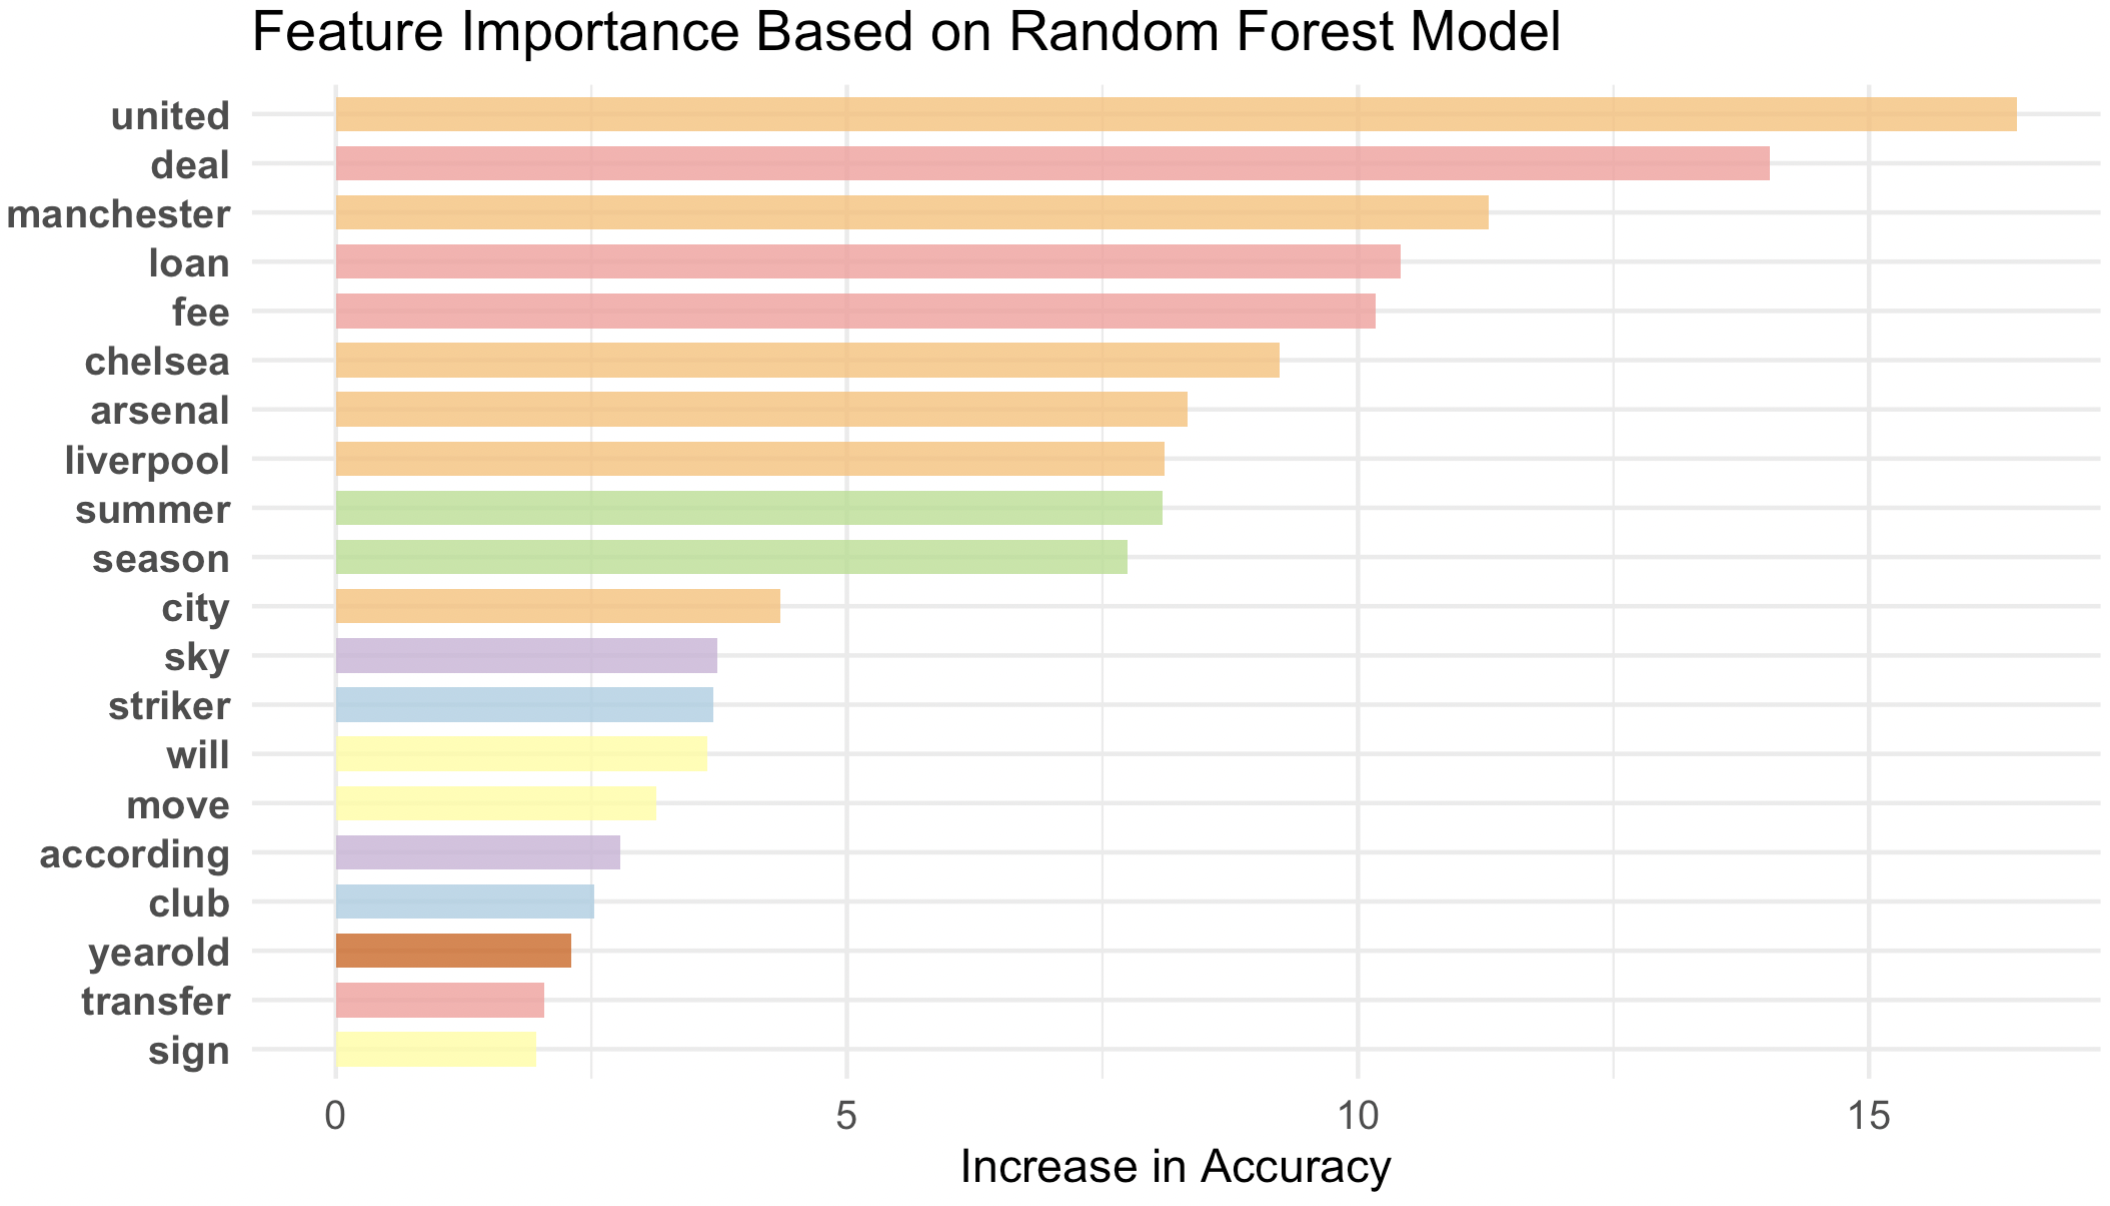
\includegraphics[width=.8\textwidth]{figs/cont_acc.png}
    \caption{
       Increased accuracy for content
    }\label{fig:cont_acc}
\end{figure}

When using only the rumor source as a feature, we construct a random forest model to evaluate its contribution to increased accuracy (i.e., the proportion of each feature's influence on model accuracy), as shown in \autoref{fig:source_acc}.

The reliability of media sources tends to be polarized, with some sources being highly credible and others being notably unreliable. This distinct variation in source reliability makes it a more effective predictor for rumor accuracy.

% 单独用谣言来源作为特征,构建随机森林模型,计算 increased accuracy(每个特征对 accuracy 的共享),如\autoref{fig:source_acc}
% 这些媒体通常是很可靠的或很不可靠的,更容易成为预测依据。

\begin{figure}[ht]
    \centering
    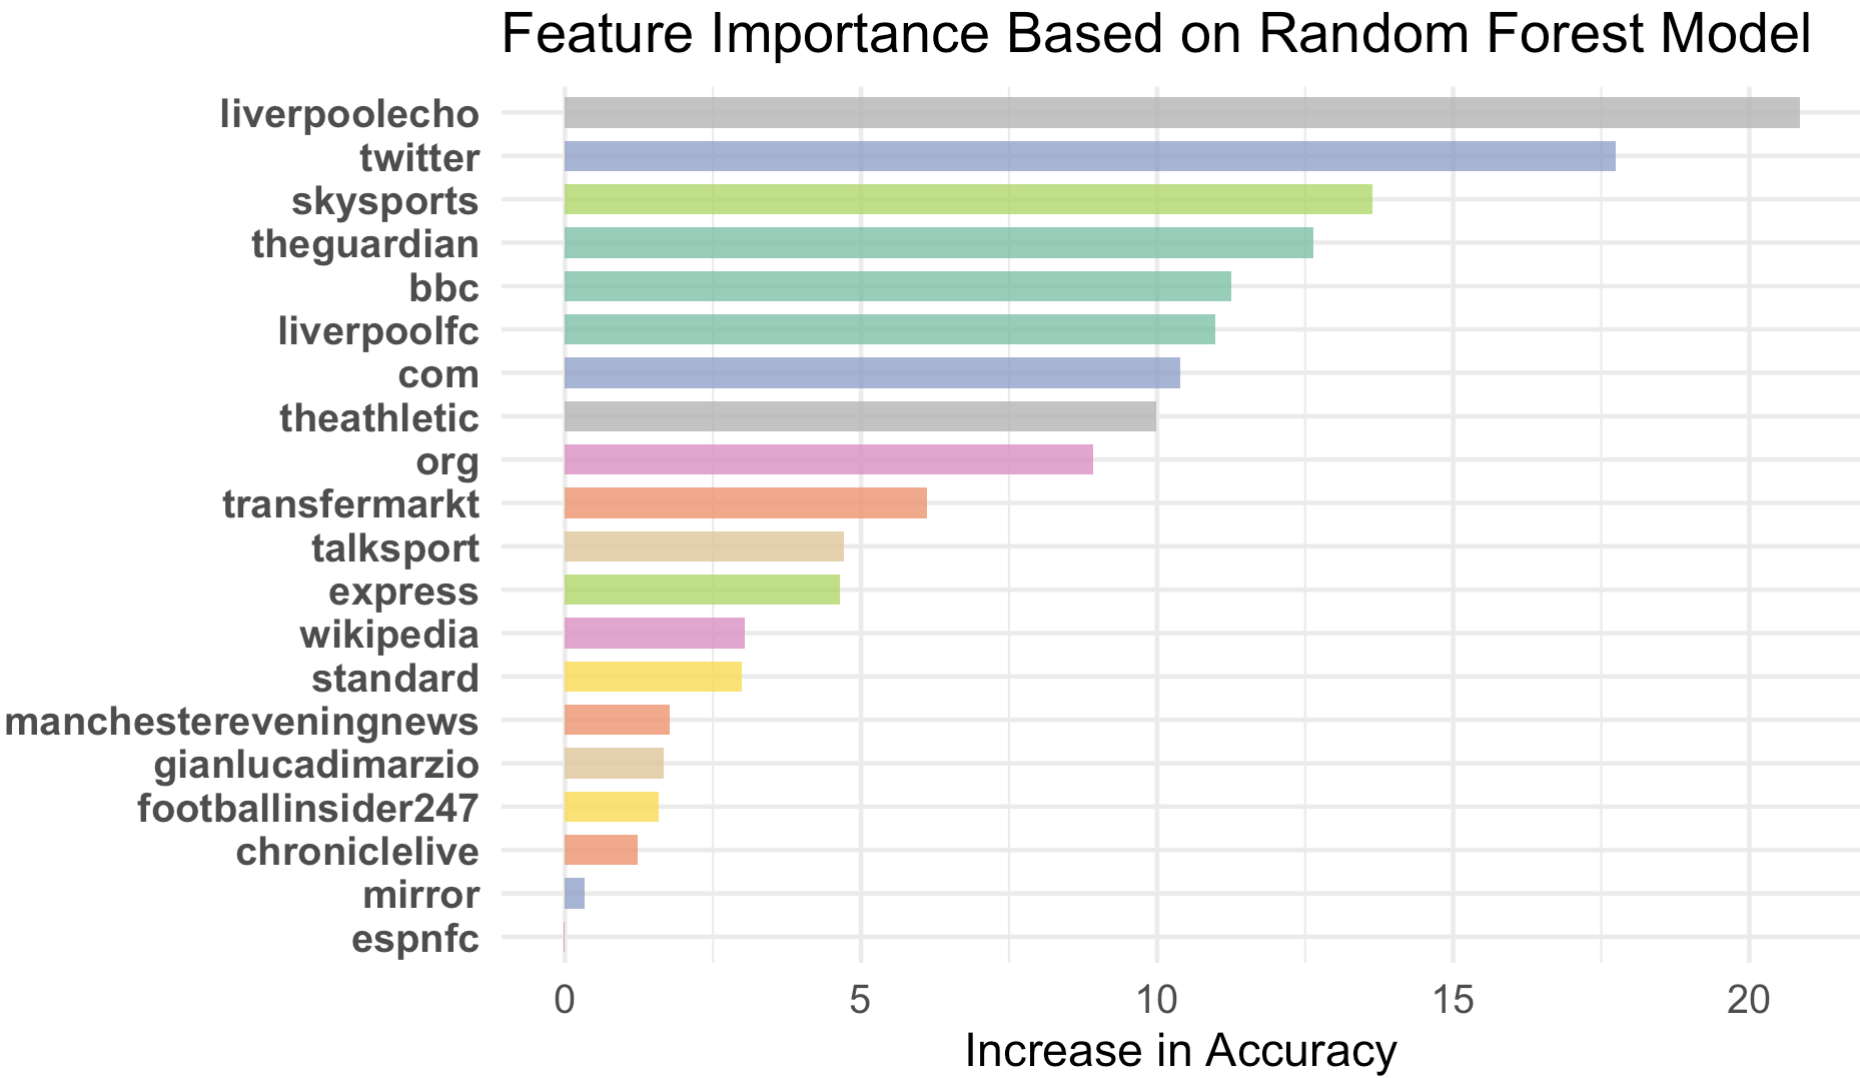
\includegraphics[width=.8\textwidth]{figs/source_acc.png}
    \caption{
       Increased accuracy for source
    }\label{fig:source_acc}
\end{figure}



\subsubsection{Others}

Through experimentation, we observed that both the nationality of the rumor publisher and the player’s position also contribute to the accuracy of subsequent predictions. As a result, we have incorporated these two features into the model.

% 我们通过实验发现,谣言发布者国籍 nationality、球员位置 position 同样有助于后续预测,故将这两类特征也包含进来。

\subsection{Prediction}

Figure \ref{fig:pred_pipe} illustrates the prediction pipeline. After aligning the data, the features are categorized into three types based on their data formats:

\begin{itemize} 
    \item \textbf{String text features:} These include the rumor content and the rumor source. These features undergo preprocessing, such as stopword removal, and are then transformed into feature matrices. Sparse entries are eliminated to reduce model complexity and accelerate the training process. 
    \item \textbf{Numeric features:} These consist of attributes such as the rumor’s publication month and GPT-confidence. These features are directly used in their numeric form for model training. 
    \item \textbf{Categorical features:} These include categorical variables such as the nationality of the rumor publisher and the player's position. Depending on the model, these features may be treated as categorical variables (e.g., in random forest models) or transformed into matrices (e.g., in SVM or ElasticNet models).
\end{itemize}


% 图 \ref{fig:pred_pipe} 是预测的pipeline。数据经过对齐后,根据数据类型的不同将特征分为三类:


% \begin{enumerate}
%     \item 字符串文本类型,包括谣言内容 content及谣言来源 source,该类特征通过进一步清洗(如删除 stopwords 等),转化为 matrix,并移除稀疏相以减小模型复杂度、加快训练速度
%     \item 数值型,包括谣言发布月份 month 及谣言可信度 GPT-conf,该类特征作为数值型直接用于训练
%     \item 单个单词字符型,包括谣言发布者国籍 nationality、球员位置 position。视模型的不同,该类特征可以是因子型(如随机森林模型),或转化为矩阵(如SVM、ElasticNet)
% \end{enumerate}


Considering the data imbalance, we performed downsampling to balance the number of positive and negative samples. A model without training would achieve an accuracy of around 50\%.

Finally, we randomly partitioned the data into training and testing sets, with a 7:3 ratio.

% 考虑到数据是不平衡的,我们通过降采样使得正负样本数目接近。此时没训练的模型可以达到 50\% 的准确率。

% 最后,我们将数据随机划分为 7:3 的比例,分别用于训练和测试。


\begin{figure}[ht]
    \centering
    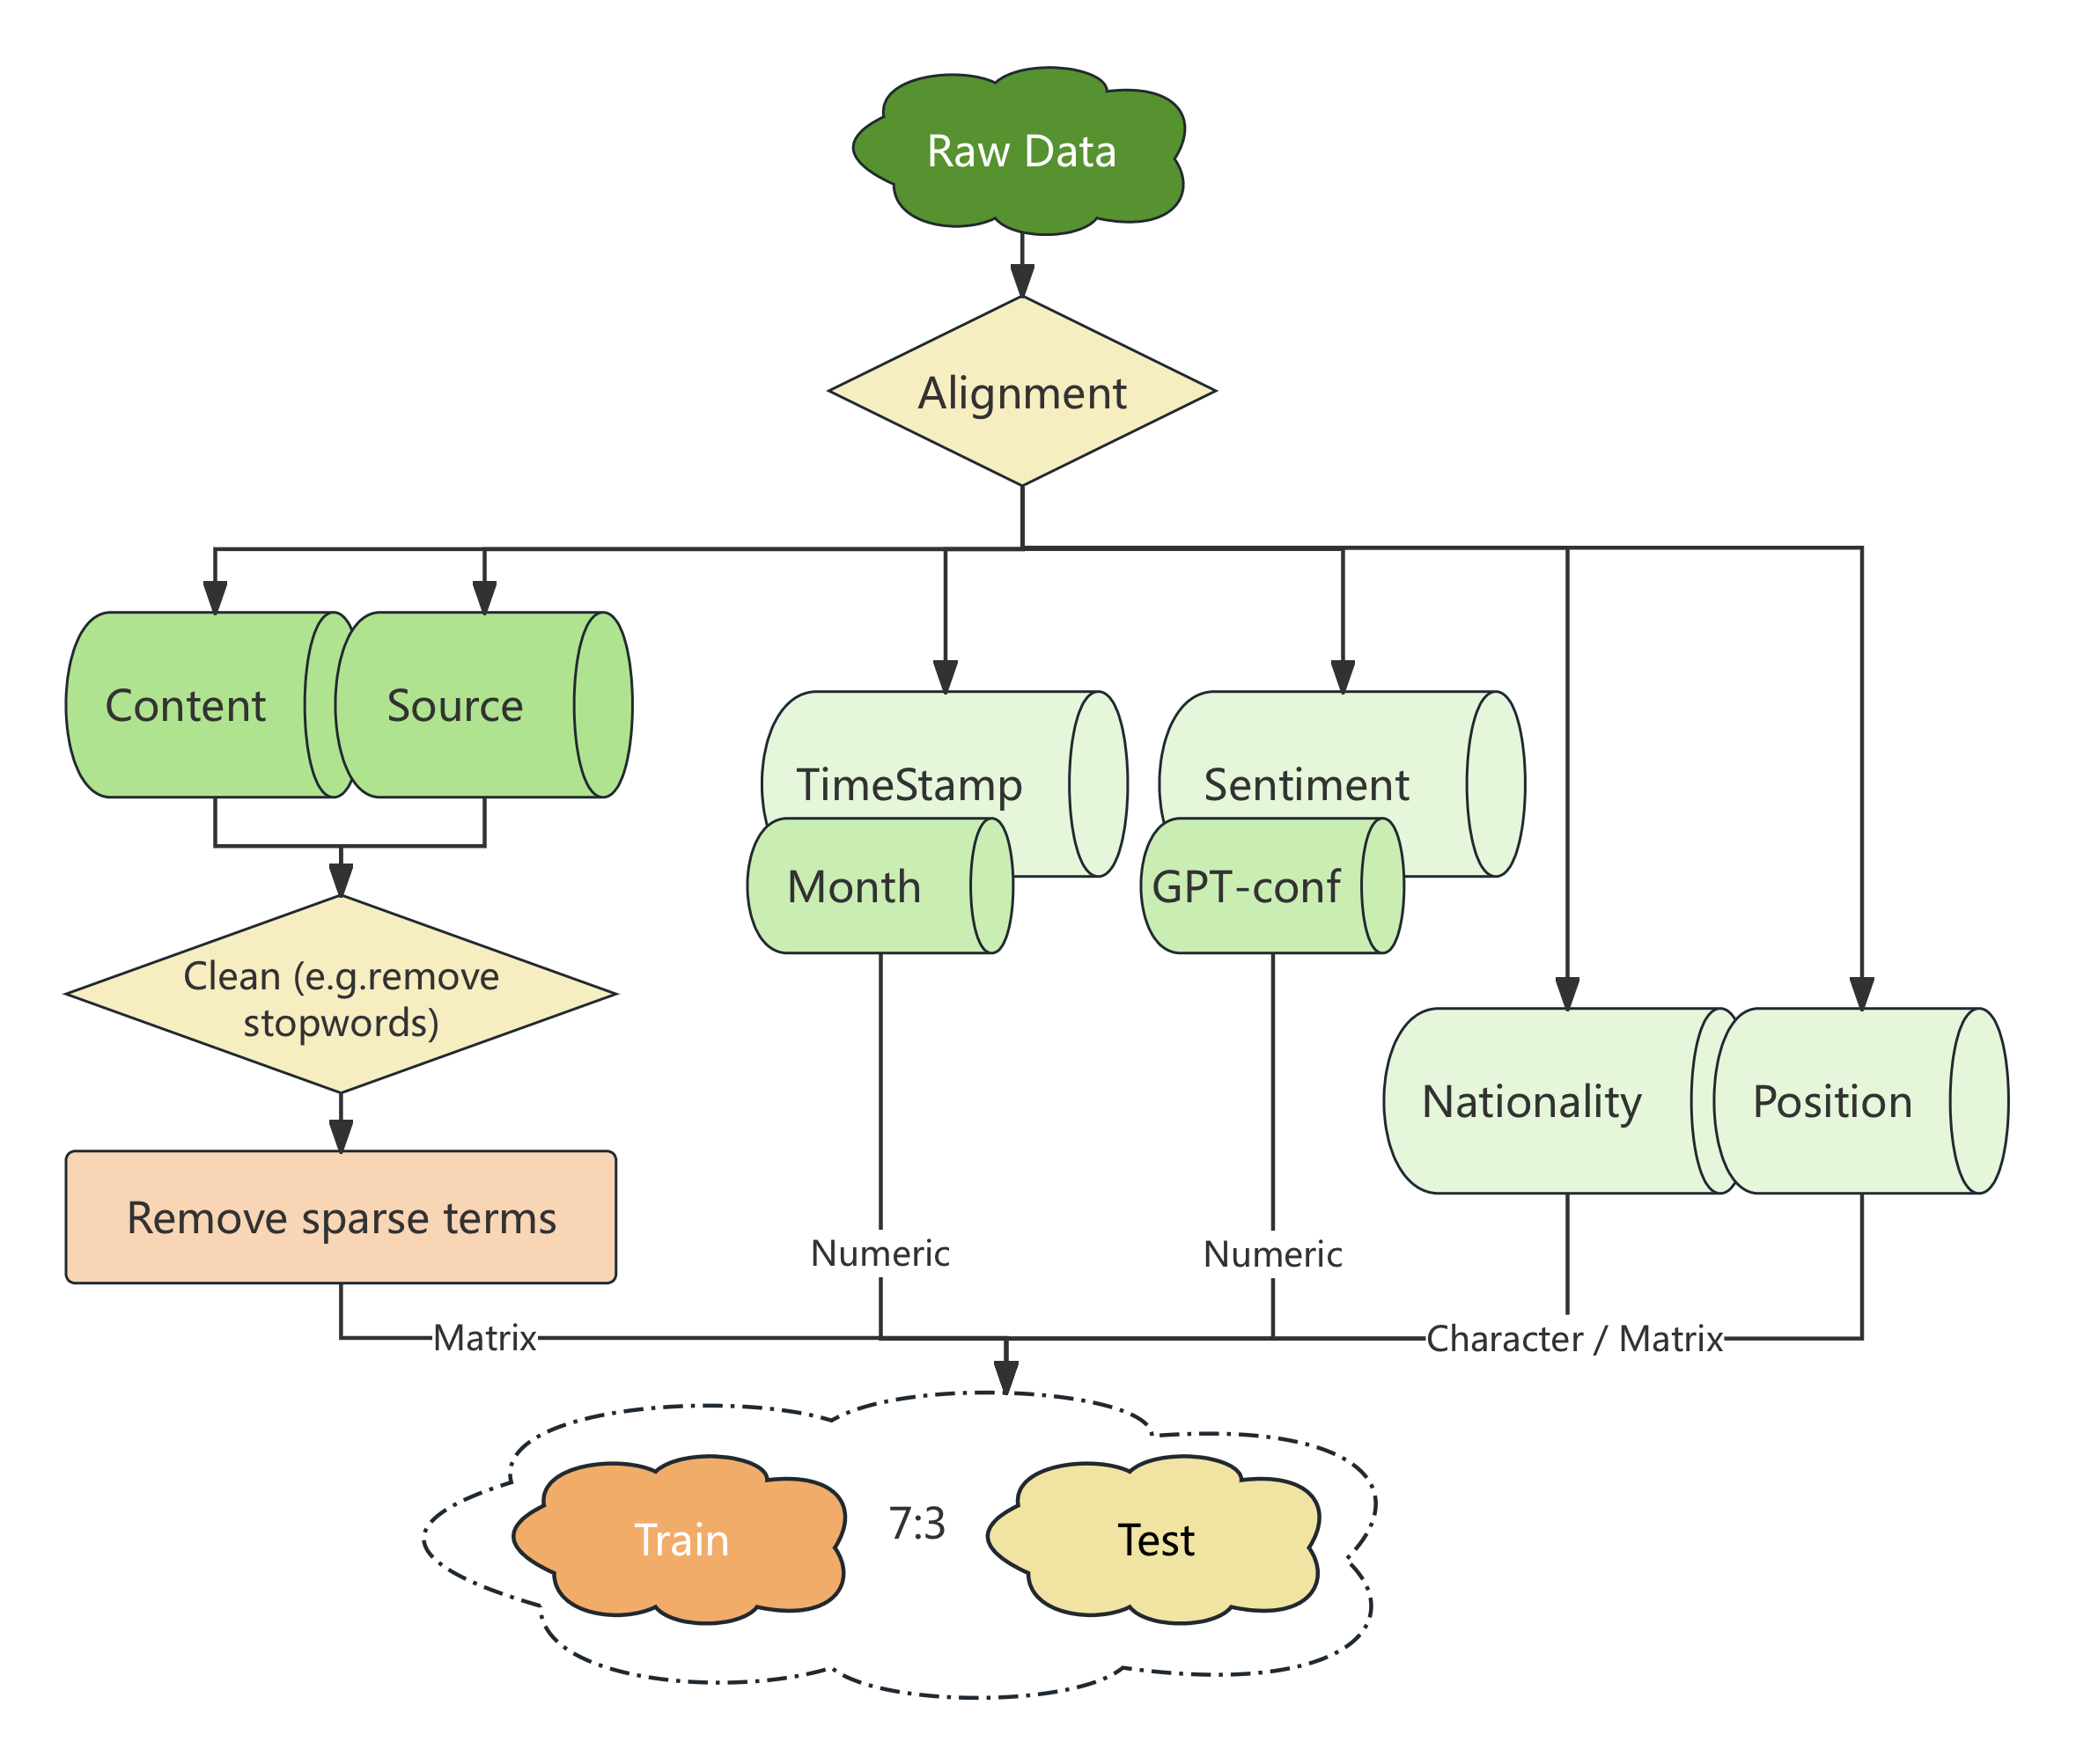
\includegraphics[width=.7\textwidth]{figs/pred_pipe.png}
    \caption{
        Pipeline for prediction
    }\label{fig:pred_pipe}
\end{figure}


\subsubsection{SVM}

SVM is a supervised machine learning algorithm used for classification and regression tasks. It aims to find the optimal hyperplane that maximizes the margin between different classes in the feature space. The problem can be formulated as the following optimization problem:

\[
\max_{\boldsymbol{\alpha}} \left[ \sum_{i=1}^N \alpha_i - \frac{1}{2} \sum_{i=1}^N \sum_{j=1}^N \alpha_i \alpha_j y_i y_j K(x_i, x_j) \right],
\]
\[
\alpha_i \geq 0,\quad\sum_{i=1}^N \alpha_i y_i = 0,\quad\alpha_i \leq C,\,\forall i.
\]

Key Parameters:

\begin{itemize} 
    \item \textbf{Kernel Function: radical} - The kernel function $K(x_i, x_j)$ is used to capture non-linear relationships between the data points. In this case, the Radial Basis Function (RBF) kernel is employed, which maps the data into a higher-dimensional space where it becomes easier to find a linear hyperplane.
    \item \textbf{Cost C: 3} - The cost parameter $C$ controls the trade-off between achieving a low margin error and ensuring that the decision boundary is as smooth as possible. A value of $C=3$ was selected based on parameter tuning, which aims to balance overfitting and underfitting.
\end{itemize}

% kernel: radical,捕捉非线性特征
% Cost:3,调参获得

\subsubsection{ElasticNet}

Logistic regression is a statistical method used for binary classification, which models the probability that a given input belongs to a particular class. The objective function, including regularization, is given by:

\[
\mathcal{L}(\beta) = \sum_{i=1}^{n} \left[ y_i \log(p_i) + (1 - y_i) \log(1 - p_i) \right]+ \lambda \left( \alpha \sum_{j=1}^{p} |\beta_j| + \frac{1}{2} (1 - \alpha) \sum_{j=1}^{p} \beta_j^2 \right).
\]

Here, $p_i$ represents the predicted probability for each data point, $y_i$ is the actual label (either 0 or 1), and $\beta_i$ are the model parameters. The regularization term ensures that the model doesn't overfit the training data.

Key parameters:

\begin{itemize}
    \item \textbf{Family: binomial} — indicating a binary classification problem.
    \item \textbf{Lambda: auto} — automatically selected during model training, often via cross-validation.
    \item \textbf{Alpha: 0.5} — a parameter that controls the mix between L1 regularization (Lasso) and L2 regularization (Ridge), set to 0.5 based on tuning for optimal performance.
\end{itemize}

The model aims to balance between minimizing the log-likelihood of the logistic regression and the regularization term, which helps prevent overfitting by penalizing large model coefficients.

% Family: binomial
% Lambda: auto,自动获得 % may add a figure
% Alpha: 0.5,调参获得


\subsubsection{Random Forest}

Random Forest is an ensemble learning method used for classification and regression tasks. It builds multiple decision trees and merges them together to produce a more accurate and stable prediction. Each tree in the forest is trained on a random subset of the data, with each node split based on a random subset of features, which helps reduce overfitting and increases generalization.

Key parameters:

\begin{itemize}
    \item \textbf{NTree: 300} — The number of trees in the forest. In this case, 300 trees are used to improve the model's performance and stability. Increasing the number of trees typically reduces variance and enhances accuracy, but comes with a computational cost.
\end{itemize}

% NTree: 300 % may add a figure


% \begin{tikzpicture}[scale=0.6]
%   \foreach \y [count=\n] in {
%       {74,25,39,20,3,3,3,3,3},
%       {25,53,31,17,7,7,2,3,2},
%       {39,31,37,24,3,3,3,3,3},
%       {20,17,24,37,2,2,6,5,5},
%       {3,7,3,2,12,1,0,0,0},
%       {3,7,3,2,1,36,0,0,0},
%       {3,2,3,6,0,0,45,1,1},
%       {3,3,3,5,0,0,1,23,1},
%       {3,2,3,5,0,0,1,1,78},
%     } {
%       % column labels
%       \ifnum\n<10
%         \node[minimum size=6mm] at (\n, 0) {\n};
%       \fi
%       % heatmap tiles
%       \foreach \x [count=\m] in \y {
%         \node[fill=yellow!\x!purple, minimum size=6mm, text=white] at (\m,-\n) {\x};
%       }
%     }

%   % row labels
%   \foreach \a [count=\i] in {a,b,c,d,e,f,g,h,i} {
%     \node[minimum size=6mm] at (0,-\i) {\a};
%   }
% \end{tikzpicture}